\section{Experiments}

We evaluate \method{} in two stages. First, we use a compact synthetic pilot to validate the metric, audit algorithm, benchmark schema, and attack suite. Second, we run a repeated submission-scale harness with a real-corpus FEVER RAG retain set, natural FEVER evidence deletion cases, simulated fine-tuning memories, and a hybrid RAG-to-derivative setting. The repeated harness spans five random seeds, three deletion-target sizes, three audit budgets, and the reviewer-response black-box/counterfactual modes, producing 6,840 audit-result rows.

\textbf{Tracks.}
The \emph{RealRAG} track loads FEVER claims and evidence passages as the retain corpus, injects synthetic private deletion targets, and evaluates provenance-guided deletion, index-only deletion, shadow-copy deletion, cache-not-purged deletion, and backdoor-triggered RAG leakage. The \emph{NaturalFEVER} track treats public FEVER evidence passages themselves as deletion-request units, then audits whether raw evidence, citation caches, summaries, or answer-only paraphrases still influence behavior after removal. The \emph{FineTuneSim} track models residual adapter memory under filtered retraining, gradient-ascent unlearning, negative fine-tuning, adapter replacement failure, and over-unlearning. The \emph{HybridReal} track combines FEVER-style RAG retention with private derivatives that survive through synthetic examples, cache artifacts, graph-pivot expansion, or model-side behavior.

\input{../Third-Best-Data-Centric-Unlearning/submission_tables/submission_table1_audit_summary}

Table~\ref{tab:submission_audit} summarizes repeated failure detection. The \method{} rows use the two-sample clean-counterfactual statistic $\hat R_{\mathrm{cf}}$ for pass/fail decisions; the other columns are diagnostic localizers. Full \method{} detects all configured RealRAG, NaturalFEVER, and HybridReal failures and 72.2\% of FineTuneSim failures with zero false alarms under the conservative counterfactual operating point. Exact-match, canary-only, and retriever-hit audits each miss important channels: exact matching misses retrieval-only and paraphrase failures, canary-only auditing misses natural data without canaries and canary-suppression failures, and retriever-hit auditing misses model-side fine-tuning residues.

\begin{table*}[t]
\centering
\caption{Headline counterfactual deletion results using the two-sample $\hat R_{\mathrm{cf}}$ statistic.}
\label{tab:cf_headline}
\resizebox{\textwidth}{!}{%
\begin{tabular}{llllllllll}
\toprule
Track & Mean Rhat Cf & Mean Ucb Cf & Mean Floor & Floor Normalized Risk & Delta & Tolerance & Failure Detection Rate & False Alarm Rate & N \\
\midrule
FineTuneSim & 0.2444 & 0.6399 & 0.508 & 0.2501 & 0.05 & 0.05 & 0.7222 & 0.0 & 225 \\
HybridReal & 0.5667 & 0.8279 & 0.508 & 0.6335 & 0.05 & 0.05 & 1.0 & 0.0 & 225 \\
NaturalFEVER & 0.3056 & 0.6842 & 0.5068 & 0.3428 & 0.05 & 0.05 & 1.0 & 0.0 & 180 \\
RealRAG & 0.2445 & 0.6648 & 0.508 & 0.307 & 0.05 & 0.05 & 1.0 & 0.0 & 225 \\
\bottomrule
\end{tabular}%
}
\end{table*}


Table~\ref{tab:cf_headline} reports the counterfactual statistic that underlies the revised definition. We use $\delta=0.05$ and a floor-normalized excess-risk tolerance of $0.05$; the raw UCB is reported beside the confidence floor so the operating rule is numerically auditable. Clean provenance-guided deletion has zero empirical clean-vs-post distance before the Hoeffding floor, while configured failures have positive $\hat R_{\mathrm{cf}}$ values. Under matched budgets (supplement), graph-adaptive allocation most improves FineTuneSim, where residual adapter memory is concentrated in fewer target--channel arms, and matches uniform allocation on the easier RAG and hybrid failures.

\begin{table*}[t]
\centering
\caption{Mid-size RealRAG scaling check on a 5,000-record FEVER retain corpus.}
\label{tab:mid_size_scaling}
\resizebox{\textwidth}{!}{%
\begin{tabular}{llllllllllll}
\toprule
Regime & Track & Audit Method & Retain Corpus N & Deletion Targets & Budget & Failure Detection Rate & False Alarm Rate & Mean Rhat Cf & Mean Ucb Cf & Floor Normalized Risk & N \\
\midrule
mid-size RealRAG retain corpus & RealRAG & ADCU & 5000 & 6 & 48 & 1.0 & 0.0 & 0.1334 & 0.5548 & 0.2152 & 5 \\
mid-size RealRAG retain corpus & RealRAG & ADCU-BlackBox & 5000 & 6 & 48 & 1.0 & 0.0 & 0.1276 & 0.5548 & 0.2152 & 5 \\
mid-size RealRAG retain corpus & RealRAG & ADCU-NoValuation & 5000 & 6 & 48 & 1.0 & 0.0 & 0.1334 & 0.5548 & 0.2152 & 5 \\
mid-size RealRAG retain corpus & RealRAG & ADCU-RetrievalOffCF & 5000 & 6 & 48 & 1.0 & 0.0 & 0.1334 & 0.5548 & 0.2152 & 5 \\
mid-size RealRAG retain corpus & RealRAG & CanaryOnly & 5000 & 6 & 48 & 0.0 & 0.0 & 0.1334 & 0.5225 & 0.1582 & 5 \\
mid-size RealRAG retain corpus & RealRAG & ExactMatch & 5000 & 6 & 48 & 0.0 & 0.0 & 0.1334 & 0.5414 & 0.1917 & 5 \\
mid-size RealRAG retain corpus & RealRAG & RetrieverHit & 5000 & 6 & 48 & 0.0 & 0.0 & 0.1334 & 0.5225 & 0.1582 & 5 \\
mid-size RealRAG retain corpus & RealRAG & UniformProbes & 5000 & 6 & 48 & 1.0 & 0.0 & 0.1334 & 0.5548 & 0.2152 & 5 \\
\bottomrule
\end{tabular}%
}
\end{table*}


Table~\ref{tab:mid_size_scaling} adds one mid-size data point: a RealRAG audit over a 5,000-record FEVER retain corpus with the same deletion and clean-reference protocol. This is not a new large-model training result, but it checks that the leakage and audit behavior are not an artifact of a few hundred retained records. The result supports the interpretation that small-data and mid-size RAG leakage differ by degree rather than by a sharp cliff.

These labels should be read carefully. The synthetic private tracks are stress tests with configured failure modes, not independent proof that the same rate holds for arbitrary private deployments. To avoid circularity, the diagnostic channels are not the formal failure definition: when a clean reference is available, we also run the two-sample distinguishability test between $S_-$ and $S_{\mathrm{clean}}$, and the channel scores are used to localize why the systems differ. NaturalFEVER and the redacted human-adjudicated cases reduce but do not eliminate the benchmark-design gap.

The full residual-channel, budget, scorer-validation, black-box, intervention, robustness, attack-suite, LoRA, DenseRAG, TOFU, probe-ablation, and per-seed uncertainty tables are in the supplement, keeping the main paper focused on the audit definition, algorithm, and headline evidence. The tolerance sweep (Fig.~\ref{fig:tolerance_roc}) also explains the apparent discrepancy between zero false alarms at the configured operating point and larger false-alarm rates in aggressive settings: the raw UCB contains the Section~4 confidence floor, so a tolerance set near or below that floor can reject clean systems with zero empirical leakage. The main decision rows therefore use the floor-normalized excess-risk tolerance, and the sweep is reported as an ROC-style calibration view separate from formal pass/fail.

\begin{figure}[t]
\centering
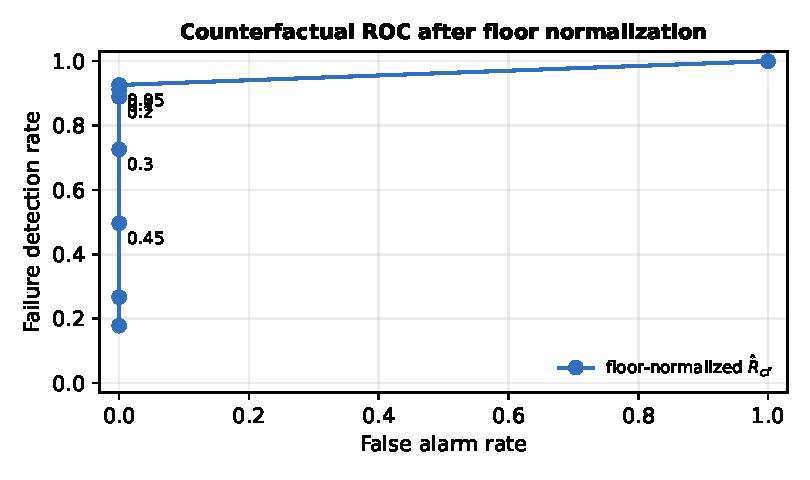
\includegraphics[width=\columnwidth]{figures/adcu_pdf/tolerance_detection_false_alarm.pdf}
\caption{Calibration view from the tolerance sweep with 95\% binomial uncertainty bands for detection rates. Lower tolerances increase sensitivity but can reject clean systems because the raw UCB includes a confidence floor.}
\label{fig:tolerance_roc}
\end{figure}

The natural-data audit uses public FEVER evidence passages as requested deletion units and records whether risk is mediated by citation caches, summary derivatives, or answer-only paraphrases. Redacted human adjudication bridges synthetic private traces and public RAG evidence without printing sensitive-looking strings in the paper body. We still treat realistic private-text deletion as an empirical limitation rather than a solved claim: the current manuscript demonstrates public natural evidence plus redacted adjudication, while a larger externally labeled private-text audit remains the next acceptance-critical experiment. Per-method HybridReal detection and the audit-budget--detection tradeoff are reported in the supplement.

The attack suite is designed to make weak audits pass while residual dependence remains through paraphrases, chunk boundaries, shadow copies, synthetic derivatives, adapter residues, evaluation evasion, retriever-reranker disagreement, retain-neighbor over-unlearning, multi-hop reconstruction, triggered RAG leakage, graph-pivot reconstruction, and watermark suppression. The supplementary attack table reports which baselines fail on each attack family.

\subsection{Advanced LoRA-SFT and DenseRAG Experiments}

We next add stronger adapter and retrieval experiments. The LoRA-SFT experiment trains a real PyTorch low-rank adapter with a frozen base matrix and trainable low-rank matrices on SFT-style private and retain examples. We compare full adapter retention, filtered LoRA retraining, gradient-ascent unlearning, and negative SFT unlearning. We also run cached HuggingFace/PEFT validations: a tiny DistilBERT LoRA sequence-classification smoke test, SmolLM2-135M causal-LM LoRA across three seeds, Qwen2.5-0.5B causal-LM LoRA across three seeds, and a larger Qwen2.5-0.5B LoRA run on a compact public TOFU-style forget/retain split~\cite{maini2024tofu}. The pretrained causal-LM runs compare filtered retraining, gradient-ascent, negative SFT, NPO with a reference-model correction, and SimNPO-style unlearning~\cite{zhang2024npo}. The DenseRAG experiment evaluates TF-IDF retrieval, SVD dense retrieval, cached MiniLM sentence-transformer retrieval, E5-base-v2 retrieval~\cite{wang2022textembeddings}, BGE-small retrieval, and a local cross-encoder-style reranker trained over query-document overlap features.

The advanced results are intentionally summarized in prose here and tabulated in the supplement with bootstrap intervals, seed counts, deletion-target counts, probe budgets, and runtime notes. In LoRA-SFT, PEFT-LoRA, Pretrained-LoRA, and Qwen-TOFU-LoRA, \method{} detects configured model-side residual failures while retriever-only auditing detects none. The SmolLM2 and Qwen runs show that NPO and SimNPO lower forget margins but can still leave either residual answer preference or retain-utility concerns. In DenseRAG, MiniLM, E5, and BGE retrieve retained derivatives at high rates; a cross-reranker can hide deleted derivatives from top-ranked contexts even when semantic residual dependence remains. Probe-family ablations confirm the same pattern: direct and paraphrase probes are strongest for adapter memory, retrieval probes are strongest for DenseRAG, extraction-only auditing is incomplete, and the full audit is the only consistently high-coverage configuration.

\begin{figure}[t]
\centering

\includegraphics[width=\columnwidth]{figures/adcu_pdf/provenance_case.pdf}
\caption{Case-study provenance graph. Gray marks the removed raw chunk, orange marks residual downstream artifacts, red marks post-deletion behavioral leakage, and green marks the audit evidence collected by \method{}.}
\label{fig:provenance_case}
\end{figure}

\subsection{Ablations}

Across repeated experiments, \method{} is compared with ADCU-NoValuation and UniformProbes. ADCU-NoValuation is a legacy ablation that removes the graph-priority signal from pre-deletion influence and provenance degree, while UniformProbes spends the probe budget evenly. The repeated RealRAG and HybridReal results show that these ablations can match full \method{} when the budget is sufficient and failures are easy to expose. In FineTuneSim, however, full \method{} improves over ADCU-NoValuation and UniformProbes, suggesting that graph-informed allocation matters most when residual dependence is concentrated in fewer model-side targets.

This evidence supports graph-informed allocation as an efficiency aid, not as a standalone superiority claim. The present implementation uses provenance degree and pre-deletion influence proxies; stronger learned influence estimators and larger external baselines are needed before claiming broad superiority over uniform allocation. We therefore scope valuation as a budget-prioritization aid and report uniform-probe results as a strong ablation rather than claiming universal sample-complexity wins. Likewise, membership-style and extraction-only rows are deliberately narrow channel baselines rather than full LiRA-style or benchmark-specific unlearning evaluators.
